\chapter{Bo}
Her er en liten "ordbok" som kan komme til hjelp:
\begin{itemize}
\item Wohnung/Leilighet/WG (Wohngemenischaft) - Bofellesskap/Kollektiv
\item Kalt Miete/warm Miete - uten og med strøm/varme inkludert i leieprisen
\item Zwischenmiete - noen som er borte for en periode og leier ut leilighet/rom
\end{itemize}

Dersom man skal ned for språkkurs og trenger bolig, har de fleste lærestedene gode løsninger.

\url{http://www.goethe.de/ins/de/ort/mue/unt/}


IKKE betal leie på forhånd, det er nok av tilfeller hvor studenter betaler leie for et semester også viser det seg at de har blitt rundlurt. 
Det er også svært lurt å ha en leiekontrakt og faktisk vite hva man signerer på.


\section{Pris}
Boligmarkedet er presset, og prisene kan være ganske høye. Skal en leie privat må en regne med å betale ca. 450 \euro{} i måneden, men det er selvsagt mulig å finne noe som er billigere. 

\section{Hvor finne leilighet}
Gjennom universitetet og studentsamskipnaden (Studentenwerk) kan en søke om plass på forskjellige studenthjem, med forskjellig standard, pris, plassering og ventetid. Hos Studentenwerk på Giselastraße kan en forhøre seg og få hjelp til dette (se hjemmeside).
På de mest populære må en kanskje venta 1,5 år, men det finnes gg steder hvor ventetiden er mindre enn et semester. En leilighet på 15 m2 med eget bad og kjøkken (10 minutter fra sentrum med U-Bahn) kan koste 250 euro. Noen av studenthjemmene ligger i sentrum, men de fleste er litt utenfor byen. De største studentbyene er Olympiadorf, Studentenstadt og Großühadern. Buss-, U-Bahn-, S-Bahn- og Straßüenbahn(trikk)-nettverket er så godt utbygd at avstandene for de fleste ikke blir noe problem. Alt som du kan nå med U-Bahn er bra, S-Bahn dekker et meget stort område, så de ytre stasjonene kan være et stykke utenfor sentrum.

\url{http://www.studentenwerk-muenchen.de/wohnen/}\\
\url{http://www.studentenwg.de}\\
\url{http://www.wg-gesucht.de}





\section{Når bør jeg begynne å lete?}
Bolig er noe av det som kan være litt kinkig å organisere (i hvert fall ifra Norge). Et godt tips: Vær tidlig ute! Altså ihvertfall en måned før studiestart.


\begin{figure}[h]
\center
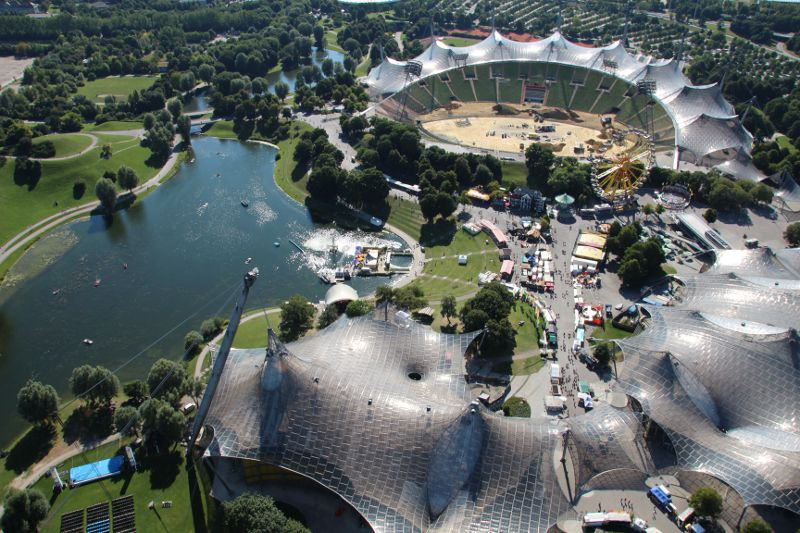
\includegraphics[width=0.30\textwidth]{./gfx/olympia}
\caption{Olympiapark ble bygget til OL i 1972}
\end{figure}


\section{Typer bomuligheter}
Det er helt smak og behag hva som er den beste løsningen for hver enkelt person. Wohngemeinschaft/WG eller kollektiv som det heter på norsk er ofte en mer sosial løsning enn å bo alene. Det kan innebære støy og andre plager, men er billigere og som sagt mer sosialt enn å bo alene. Pris rundt 400 \euro{}

Studentenheim er nok den billigste løsningen og man har som regel en egen, noe mindre, hybel. Her bør man være litt på vakt, det er flere katolske og andre former for studentenheim som har egne regler, angående besøk av kjærester og annet.
Ventelistene er ofte lange og man må vente opptil et til to år før det er en ledig hybel.
Pris rundt 300 \euro{}

Man kan også velge å bo alene, den dyreste og minst sosiale løsningen. Passer kanskje til den som er noe mer reservert, men kan fort bli litt ensomt og lite kontakt med tyskere . På den andre siden er man bedre vernet fra bråk og forstyrelser.
Pris rundt 450 \euro{}

Hva skal man velge? det må du finne ut selv!


